\section{Quality vs output length}
\label{app:quality} Figure~\ref{fig:quality} shows what happens to quality when output length is
forced. The dense AR-3B's 9-field F1 is flat at \arThreeBFnine{} from
$L{=}\canvasLength$ to $L{=}512$ --- not because the model is invariant, but
because first-object-wins parsing (defect 3, Appendix~\ref{app:defects})
discards the tokens past the first JSON object. At $L{=}128$ the AR model
retains \arFOneTwentyEight{} F1 and \arValidTwentyEight\% schema validity,
while the diffusion model falls to \dgFOneTwentyEight{} and
\dgValidTwentyEight\%. \begin{figure}[t]
\centering
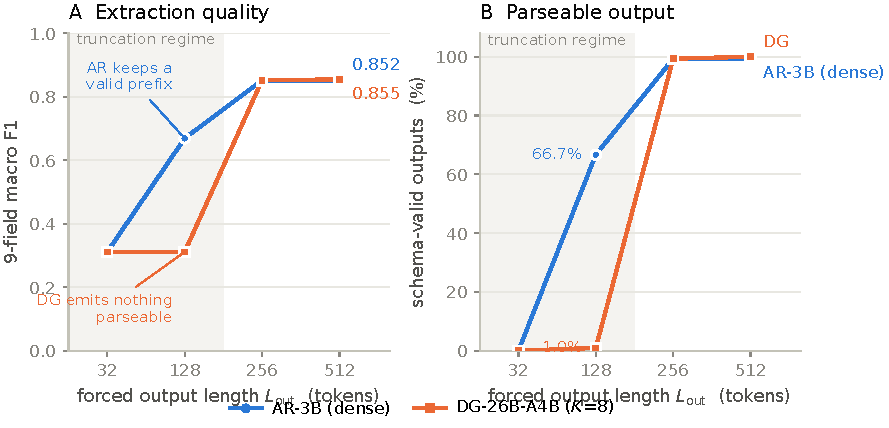
\includegraphics[width=\linewidth]{figures/fig5_quality_vs_length.pdf}
\caption{Quality and schema validity as a function of forced output length
(BGL, $n{=}300$ per cell; AR arm is the dense AR-3B baseline, Qwen2.5-3B).
AR-3B F1 is flat from $L{=}256$ to $L{=}512$ because first-object-wins
parsing discards the rambled continuation. The diffusion model's quality
rises with $L$ and then plateaus.}
\label{fig:quality}
\end{figure} The diffusion model degrades gracefully against a \emph{time} budget and
catastrophically against an \emph{output-length} budget. Which one an
application faces decides which architecture is safer.
